\documentclass[11pt]{article}
\usepackage[utf8]{inputenc}

\usepackage{latexsym}
\usepackage{amssymb,amsmath}
\usepackage{graphicx}
\usepackage{sgame}
\usepackage{color}
\usepackage{authblk}

%\usepackage{indentfirst}
\usepackage[toc,page]{appendix}
\renewcommand{\appendixname}{Appendix}
\renewcommand{\appendixtocname}{Appendix}
\renewcommand{\appendixpagename}{Appendix}

\usepackage[hidelinks]{hyperref}
\usepackage{empheq}
\usepackage{blkarray}
\usepackage{cancel}
\usepackage{enumerate}
\usepackage{times}
\usepackage{array}
\usepackage{lscape}

\usepackage[margin=.75in]{geometry}
\newcommand{\newword}[1]{\textbf{\emph{#1}}}

%Arrows
\newcommand{\into}{\hookrightarrow}
\newcommand{\onto}{\twoheadrightarrow}

%Macros
\newcommand{\isom}{\cong} %The isomorphism symbol
\newcommand{\union}{\cup}
\newcommand{\intersection}{\cap}
\newcommand{\bigunion}{\bigcup}
\newcommand{\bigintersection}{\bigcap}
\newcommand{\disjointunion}{\sqcup}
\newcommand{\bigdisjointunion}{\bigsqcup}

\newcommand\numberthis{\addtocounter{equation}{1}\tag{\theequation}}

%Some multiletter functions
\DeclareMathOperator{\Hom}{Hom}
\DeclareMathOperator{\Ext}{Ext}
\DeclareMathOperator{\End}{End}
\DeclareMathOperator{\Tor}{Tor}
\DeclareMathOperator{\Ker}{Ker}
\DeclareMathOperator{\CoKer}{CoKer}
\DeclareMathOperator{\Spec}{Spec}
\DeclareMathOperator{\Proj}{Proj}
\renewcommand{\Im}{\mathop{\mathrm{Im}}}
%Their calligraphic versions; use these for the sheaf constructions
\DeclareMathOperator{\HHom}{\mathcal{H} \textit{om}}
\DeclareMathOperator{\EExt}{\mathcal{E} \textit{xt}}
\DeclareMathOperator{\EEnd}{\mathcal{E} \textit{nd}}
\DeclareMathOperator{\TTor}{\mathcal{T} \textit{or}}
\DeclareMathOperator{\KKer}{\mathcal{K}\textit{er}}
\DeclareMathOperator{\CCoKer}{\mathcal{C} \textit{o}\mathcal{K} \textit{er}}
\newcommand{\IIm}{\mathop{\mathcal{I} \textit{m}}}
\newcommand{\ccH}{\mathscr{H}} %The very curly H

\DeclareMathOperator{\sss}{\mathrm{sunny}}
\DeclareMathOperator{\rrr}{\mathrm{rainy}}
\DeclareMathOperator{\hhh}{\mathrm{hot}}
\DeclareMathOperator{\ccc}{\mathrm{cold}}


%This makes alternating tensors look right in displayed equations
\newcommand{\Alt}{\bigwedge\nolimits}

%Blackboard bold letters

\renewcommand{\AA}{\mathbb{A}}
\newcommand{\BB}{\mathbb{B}}
\newcommand{\CC}{\mathbb{C}}
\newcommand{\DD}{\mathbb{D}}
\newcommand{\EE}{\mathbb{E}}
\newcommand{\FF}{\mathbb{F}}
\newcommand{\GG}{\mathbb{G}}
\newcommand{\HH}{\mathbb{H}}
\newcommand{\II}{\mathbb{I}}
\newcommand{\JJ}{\mathbb{J}}
\newcommand{\KK}{\mathbb{K}}
\newcommand{\LL}{\mathbb{L}}
\newcommand{\MM}{\mathbb{M}}
\newcommand{\NN}{\mathbb{N}}
\newcommand{\OO}{\mathbb{O}}
\newcommand{\PP}{\mathbb{P}}
\newcommand{\QQ}{\mathbb{Q}}
\newcommand{\RR}{\mathbb{R}}
\renewcommand{\SS}{\mathbb{S}}
\newcommand{\TT}{\mathbb{T}}
\newcommand{\UU}{\mathbb{U}}
\newcommand{\VV}{\mathbb{V}}
\newcommand{\WW}{\mathbb{W}}
\newcommand{\XX}{\mathbb{X}}
\newcommand{\YY}{\mathbb{Y}}
\newcommand{\ZZ}{\mathbb{Z}}

%Calligraphic letters

\newcommand{\cA}{\mathcal{A}}
\newcommand{\cB}{\mathcal{B}}
\newcommand{\cC}{\mathcal{C}}
\newcommand{\cD}{\mathcal{D}}
\newcommand{\cE}{\mathcal{E}}
\newcommand{\cF}{\mathcal{F}}
\newcommand{\cG}{\mathcal{G}}
\newcommand{\cH}{\mathcal{H}}
\newcommand{\cI}{\mathcal{I}}
\newcommand{\cJ}{\mathcal{J}}
\newcommand{\cK}{\mathcal{K}}
\newcommand{\cL}{\mathcal{L}}
\newcommand{\cM}{\mathcal{M}}
\newcommand{\cN}{\mathcal{N}}
\newcommand{\cO}{\mathcal{O}}
\newcommand{\cP}{\mathcal{P}}
\newcommand{\cQ}{\mathcal{Q}}
\newcommand{\cR}{\mathcal{R}}
\newcommand{\cS}{\mathcal{S}}
\newcommand{\cT}{\mathcal{T}}
\newcommand{\cU}{\mathcal{U}}
\newcommand{\cV}{\mathcal{V}}
\newcommand{\cW}{\mathcal{W}}
\newcommand{\cX}{\mathcal{X}}
\newcommand{\cY}{\mathcal{Y}}
\newcommand{\cZ}{\mathcal{Z}}


\DeclareMathOperator{\ord}{ord}
\DeclareMathOperator{\inte}{int}
\DeclareMathOperator{\nhd}{nhd}

\newcommand{\ds}{\displaystyle}
\newcommand{\mc}{\mathcal}
\newcommand{\ol}{\overline}
\newcommand{\modu}{\hspace{-2mm} \mod}

\DeclareMathOperator{\inn}{Inn}
\DeclareMathOperator{\aut}{Aut}
\DeclareMathOperator{\cen}{Center}
\DeclareMathOperator{\im}{Im}
\DeclareMathOperator{\re}{Re}
\DeclareMathOperator{\id}{id}
\DeclareMathOperator{\mor}{Mor}
\DeclareMathOperator{\irr}{Irr}
\DeclareMathOperator{\sgn}{sgn}

\DeclareMathOperator{\cov}{Cov}
\DeclareMathOperator{\var}{Var}

\DeclareMathOperator{\erf}{erf}
%\DeclareMathOperator{\sgn}{sgn}
\DeclareMathOperator{\argmin}{argmin}
\DeclareMathOperator{\argmax}{argmax}

\DeclareMathOperator{\lip}{Lip}

\newcommand{\bbm}{\begin{bmatrix}}
\newcommand{\bpm}{\begin{pmatrix}}
\newcommand{\ebm}{\end{bmatrix}}
\newcommand{\epm}{\end{pmatrix}}

\newcommand{\ddx}[2]{\frac{d #1}{d #2}}
\newcommand{\ddt}[1]{\frac{d #1}{dt}}

 \newcommand{\del}[2]{\frac{\partial #1}{\partial #2}}
 \newcommand{\dsdel}[2]{\displaystyle\frac{\partial #1}{\partial #2}}
 
 \newcommand{\doubledel}[3]{\displaystyle\frac{\partial^2 #1}{\partial #2 \partial #3}}
 \newcommand{\doubledelsame}[2]{\displaystyle\frac{\partial^2 #1}{\partial #2^2}}
  
%newcommand{\ddx}[2]{\frac{d #1}{d #2}}
%\newcommand{\ddt}[1]{\frac{d #1}{dt}}

\newcommand{\dsddx}[2]{\displaystyle\frac{d #1}{d #2}}
\newcommand{\dsddt}[1]{\displaystyle\frac{d #1}{dt}}

\newcommand{\pbderiv}{\ds\del{V}{x_1} \dsddt{x_1} + \ds\del{V}{x_2} \dsddt{x_2}}

\newcommand{\ito}{It\^o \hspace{0.05mm}}
\newcommand{\itos}{It\^os \hspace{0.05mm}}

\newcommand{\gronwall}{Gr\"onwall  \hspace{0.05mm}}
\newcommand{\gronwalls}{Gr\"onwall's  \hspace{0.05mm}}

\newcommand{\tw}{d\tilde{W}_t}
\newcommand{\tws}{d\tilde{W}_s}

\bibliographystyle{plain}
\usepackage{float}


%%%%%%%%%%%%%%%%%%%%%%%%%%%
% Document-specific settings

\title{Fixed Threshold Mixing Model ({\color{red}Draft v2})}
\author{Mari Kawakatsu and Christopher K. Tokita}
\date{Last updated: \today}

\graphicspath{ {../output/Task_dist/} }
\usepackage[labelfont=bf,margin=.3in]{caption}

%%%%%%%%%%%%%%%%%%%%%%%%%%%
\begin{document}

\maketitle
\tableofcontents

\newpage
\section{Overview}

\subsection{Aim}\label{sec:aim}
Our goal is to understand how varying one or more or the parameters of the fixed threshold model (FTM) affects the behavior of single line (A or B) colonies and mixed colonies. Specifically, we are interested what parameter combinations produce the following patterns that (we think) we observe in the empirical data (Figs.~1~and~2 in Yuko's document):

\begin{itemize}
    \item \textbf{Differences in colony average behavior}: 
    In the experiment, colonies of A and B ants have different mean RMSD values. Correspondingly, we expect the model to produce \textit{different mean frequencies of task 1 performance between line A and B ants in isolation}.

    \item \textbf{Convergence of behavior between lines in the mixed case}:
    When the A and B lines are mixed in the experiment, the two genotypes appear to become behaviorally more similar. Moreover, this behavioral `contagion' is asymmetric, and the direction of convergence (i.e. whether the mean RMSD in the mixed case becomes closer to that of A alone or B alone) depends on the type of larvae. We therefore expect the model to show 1) \textit{convergence in mean frequencies of task 1 performance between line A and B ants} and 2) \textit{different asymmetries in such behavioral convergence depending on some relative property of tasks}.
    
\end{itemize}

%{\color{red}
%\subsection{The two-line fixed threshold model}
%Should I write down equations for the model?
%}

\subsection{Parameter exploration}

\subsubsection{Parameter descriptions \& base case} \label{sec:original}
Table~\ref{tab:original} summarizes the parameters used in the fixed threshold model for single-line colonies in Ulrich et al.~\cite{ulrich2018}.
\begin{table}[H] \small
  \begin{center}
    \begin{tabular}{|c|c|c|c|} 
      \hline
      \textbf{Parameter} & \textbf{Definition} & \textbf{Model values} \\ \hline
      $n$ & No. of individuals & $1\leq n \leq16$ \\ \hline
      $m$ & No. of tasks & $m = 2$ \\ \hline
      $\delta$ & Demand rate & $\delta = 0.6$  \\ \hline
      $\alpha$ & Task performance efficiency & $\alpha = m(=2) $  \\ \hline
      $\mu$ & Mean threshold & $\mu = 10$  \\ \hline
      $\sigma$ & Threshold variation & $0 \leq \sigma \leq 0.5$  \\ \hline
      $\eta$ & Threshold stochasticity & $1 \leq \eta \leq 30 $ \\ \hline
      $\tau$ & Quit probability & $\tau = 0.2$ \\ \hline
    \end{tabular}
    \caption{Parameterization of the FTM in Ulrich et al.~\cite{ulrich2018}. The parameter values are taken from Fig.~3 of the paper, on which we have based the base model for our investigation. Note that $\delta$, $\alpha$, $\mu$, and $\sigma$ can be task-specific but are assumed to be the same across tasks in \cite{ulrich2018}.}
    \label{tab:original}
  \end{center}
\end{table}

\vspace{-20pt}
Based on this, we have chosen the following parameters for the base case: $\delta = 0.6$, $\alpha = 2$, $\mu = 10$, $\sigma = 0.1$, $\eta = 7$, $\tau = 0.2$. Note that these values apply to both tasks (1 and 2) and both lines (A and B).
%For reference, the parameters values used in \cite{ulrich2018} are summarized in Table~\ref{tab:original} in Appendix~\ref{sec:original}.

\subsubsection{Varying parameters by line} 

An intuitive way to capture the inherent differences between the two lines (A and B) is to vary some of the parameters by line. Of the parameters in the model, we think that the following five might plausibly capture the phenotypic differences: \textbf{ performance efficiency $\alpha$, mean threshold $\mu$, threshold variation $\sigma$, threshold stochasticity parameter $\eta$}, and \textbf{quit probability~$\tau$}. To systematically investigate their effects, we have taken the base model and varied one of these five parameters at a time. For example, when testing the effects of varying the task efficiency $\alpha$ between the two lines, we introduced variation in $\alpha$ only ($\alpha^A = 2$, $\alpha^B = 6$) and kept all other parameter values identical the base model ($\delta = 0.6$, $\mu = 10$, $\sigma = 0.1$, $\eta = 7$, $\tau = 0.2$). Table~\ref{tab:byline} summarizes the specific values we have tested, along with corresponding biological interpretations.

\begin{table}[h] \small
  \begin{center}
    \begin{tabular}{|c|>{\centering}m{0.6in}|>{\centering}m{1.15in}|m{3.5in}|} 
      \hline
      \textbf{Parameter} & \textbf{Varied?} & \textbf{Model value(s)} & \textbf{Notes / Biological interpretation} \\ \hline
      $n$ & Fixed & $n = 4, 16$ & Based on colony sizes used in the mixing experiments \\ \hline
      $m$ & Fixed & $m = 2$ & For simplicity; no compelling reason to change from \cite{ulrich2018} \\ \hline
      $\delta$ & Fixed & $\delta = 0.6$ & Stimulus increase rate should not depend on line\\ \hline
      $\alpha$ & By line  & $\alpha^A = 2,\alpha^B = 6$ & Line B ants are more efficient than line A ants at both tasks \\ \hline
      $\mu$ & By line  & $\mu^A = 10,\mu^B = 20 $ & Line B ants have higher mean thresholds than line A ants for both tasks; creates a bimodal distribution of thresholds in the mixed case \\ \hline
      $\sigma$ & By line & $\sigma^A = 0.1, \sigma^B = 0.3$ & Line B ants have a greater range of internal thresholds than line A ants; seems unlikely since variance in RMSD does not appear to differ between lines A and B, but included for thoroughness \\ \hline
      $\eta$ & By line & $\eta^A = 7, \eta^B = 14 $ &  Line B ants respond more deterministically to both stimuli than line A ants\\ \hline
      $\tau$ & By line & $\tau^A = 0.2,\tau^B = 0.8 $ & Line B ants tend to spend less time on a given task than line A ants; could be correlated to their relative cycle lengths (A has slower cycles than B) \\ \hline
    \end{tabular}
    \caption{Varying parameters by line.\vspace{-15pt}}
    \label{tab:byline}
  \end{center}
\end{table}

\subsubsection{Varying parameters by task} 
We have also tested the effect of varying some of the parameters by task type (1 or 2) without differentiating between the two lines. 
Since all ants are identical in this case, we did not expect colonies of different compositions (A only, B only, A and B) to perform differently---and the simulations confirmed our expectation---but we have included this investigation for thoroughness.
If interested, see Appendix~\ref{sec:bytask} for details.


\section{Main results}

Here we highlight results that either show some significant behavior or we think would be of interest to you. All other results are included in the Appendix.

\subsection{Base case}

\begin{figure}[H]
	\centering
	\includegraphics[width=.4\linewidth]{{AThreshM_10.00_10.00_BThreshM_10.00_10.00_deltas_0.60_0.60_threshSlope_7_Aalpha_2.00_2.00_Balpha_2.00_2.00_quitP_0.20}.png}
	\caption{Base case. Parameter values are $\delta = 0.6$, $\alpha = 2$, $\mu = 10$, $\sigma = 0.1$, $\eta = 7$, and $\tau = 0.2$ for both tasks (tasks 1 and 2) and lines (lines A and B).}
	\label{fig:base}
\end{figure}

\subsection{Varying parameters by line only}\label{sec:byline}

\subsubsection{Varying task performance efficiency $\alpha$ by line}

\begin{figure}[H]
	\centering
	\includegraphics[width=.4\linewidth]{{New_AThreshM_10.00_10.00_BThreshM_10.00_10.00_deltas_0.60_0.60_threshSlope_7_Aalpha_2.00_2.00_Balpha_6.00_6.00_quitP_0.20}.png}
	\caption{Varying task performance efficiency ($\alpha$) by line. The parameter values are identical to those in the base case (Fig.~\ref{fig:base}) with the exception of line-specific efficiencies: $\alpha^A = 2, \alpha^B = 6$.
%	\\ \hspace{0pt}\\
%	\textbf{Observation}: 
	\vspace{-10pt}}
	\label{fig:varyalphaAB}
\end{figure}

If B ants are more efficient than A ants, we would intuitively expect B ants to spend less time performing tasks because the more efficient the ants are, the more quickly the stimuli decrease. As expected, we see that the mean task 1 performance frequency for B ants only (left third) is lower than that for A ants only (middle third).
The same pattern is observed for task 2. 
We also observe asymmetric behavioral convergence in the mixed case.
%the A and B ants become more similar in behavior in the mixed case (right third), and the mean task 1 performance frequency in the mixed case appears to be lower than the \textit{mean} of the mean task 1 performance frequencies in the single-line cases.

\subsubsection{Varying mean threshold $\mu$ by line}

\begin{figure}[H]
	\centering
	\includegraphics[width=.4\linewidth]{{AThreshM_10.00_10.00_BThreshM_20.00_20.00_deltas_0.60_0.60_threshSlope_7_Aalpha_2.00_2.00_Balpha_2.00_2.00_quitP_0.20}.png}
	\caption{Varying mean threshold ($\mu$) by line. The parameter values are identical to those in the base case (Fig.~\ref{fig:base}) with the exception of line-specific mean thresholds, $\mu^A = 10, \mu^B = 20$. 
%	\\\hspace{0pt}\\
%\textbf{Observation}: 
\vspace{-10pt}}
	\label{fig:varymuAB}
\end{figure}

Somewhat counterintuitively, changing the mean internal threshold by line \textit{does not} change the mean frequency of task 1 performance in single-line colonies. In the mixed case, however, we observe the expected increase in behavioral specialization.

\subsubsection{Varying quit probability $\tau$ by line}

\begin{figure}[H]
	\centering
	\includegraphics[width=.4\linewidth]{{AThreshM_10.00_10.00_AThreshSD_0.10_0.10_BThreshM_10.00_10.00_BThreshSD_0.10_0.10_deltas_0.60_0.60_threshSlope_7_7_Aalpha_2.00_2.00_Balpha_2.00_2.00_quitP_0.20_0.80}.png}
	\caption{Varying quit probability ($\tau$) by line. The parameter values are identical to those in the base case (Fig.~\ref{fig:base}) with the exception of line-specific quit probabilities, $\tau^A = 0.2, \tau^B = 0.8$. 
%	\\\hspace{0pt}\\
%\textbf{Observation}: 
%Higher quit probability ($\tau^B = 0.8$) means that line B ants experience greater turnover rate, which results in smaller variance in frequency of performing task 1.
%{\color{black}
%If there is a way to count the number of times the ants ``switch tasks'' (i.e. go to and from the nest), then we could measure a proxy for the average period that the ants spend on one task. The quit probability can be estimated as its inverse.}
\vspace{-5pt}}
	\label{fig:varytauAB}
\end{figure}

The higher quit probability ($\tau^B$ = $0.8$) leads to a higher turnover rate for B ants, which results in a smaller variance in the frequency of performing task 1.
{\color{black}
We are wondering if there is a way to empirically measure the quit probability.
For example, might it be possible to estimate the average period that the ants spend on one task by counting the number of times they ``switch tasks'' (i.e. go to and from the nest). Then the quit probability can be estimated as its inverse. If there is no significant difference in this quit probability proxy between A and B ants, then the variation in $\tau$ would be a biologically implausible explanation for the mixing patterns.}

\subsection{Varying parameters by both line and task}

\subsubsection{Varying task performance efficiency $\alpha$ by both line and task}
\vspace{-7pt}
\begin{figure}[H]
	\centering
	\includegraphics[width=.4\linewidth]{{New_AThreshM_10.00_10.00_AThreshSD_0.10_0.10_BThreshM_10.00_10.00_BThreshSD_0.10_0.10_deltas_0.60_0.60_threshSlope_7_7_Aalpha_2.00_6.00_Balpha_6.00_2.00_quitP_0.20_0.20}.png}
	\caption{Varying task efficiency ($\alpha$) by both line and task. The line-and-task-specific efficiencies are $\alpha^A_1 = 2,\ \alpha^A_2 = 6,\ \alpha^B_1 = 6,\ \alpha^B_2 = 2$. 
%	\\\hspace{0pt}\\
%\textbf{Observation}: 
\vspace{-10pt}
}
	\label{fig:varyalphaAB12}
\end{figure}

Similar to the case where $\alpha$ is varied by line only (Fig.~\ref{fig:varyalphaAB}), varying $\alpha$ by both line and task produces different mean frequencies of task 1 performance between A-only and B-only colonies. However, unlike in Fig.~\ref{fig:varyalphaAB}, where B-only colonies performed both tasks (1 and 2) less frequently compared to A-only colonies, here the B-only colonies perform task 2 more frequently than A-only colonies. Again, this supports our intuition that the more efficient an ant is at a task, the less time it spends performing that task.

\subsubsection{Varying mean threshold $\mu$ by both line and task}
\vspace{-7pt}
\begin{figure}[H]
	\centering
	\includegraphics[width=.4\linewidth]{{AThreshM_10.00_20.00_BThreshM_20.00_10.00_deltas_0.60_0.60_threshSlope_7_Aalpha_2.00_2.00_Balpha_2.00_2.00_quitP_0.20}.png}
	\caption{Varying mean threshold ($\mu$) by both line and task. The line-and-task-specific efficiencies are $\mu^A_1 = 10,\ \mu^A_2 = 20,\ \mu^B_1 = 20,\ \mu^B_2 = 10$.
%\textbf{Observation}: 
\vspace{-10pt}
}
	\label{fig:varymuAB12}
\end{figure}

Similar to the case where $\mu$ is varied by line only (Fig.~\ref{fig:varymuAB}), varying $\mu$ by both line and task \textit{does not} produce different mean frequencies of task 1 performance between A-only and B-only colonies. The reversed ordering of the thresholds between lines A and B (A ants have a higher mean threshold for task 2 compared to task 1, and vice versa for B ants) leads to a greater behavioral specialization in the mixed case compared to Fig.~\ref{fig:varymuAB}.

\section{Conclusions so far}

By systematically varying the parameters of the FTM, we have made progress in disentangling their effects on the model behavior in both single-line and mixed cases. Our main takeaways so far are as follows:

\begin{itemize}
	\item Varying the \textbf{task performance efficiency ($\alpha$)} by line produces 1) different mean task 1 performance frequencies in single-line colonies, analogous to different mean RMSD values observed in the experiment, and 2) convergence of behavior between lines in the mixed colonies, similar to the asymmetric behavioral ``contagion'' pattern observed in the experiment.
	
	\item Contrary to what we might expect intuitively, varying the \textbf{mean threshold ($\mu$)} by line does \textit{not} produce different mean task 1 performance frequencies. In the mixed case, however, we do observe the behavioral ``amplification'' pattern, i.e., greater behavioral specialization.

	\item Similarly, varying the \textbf{quit probability ($\tau$)} by line does \textit{not} produce different mean task 1 performance frequencies but produces the behavioral amplification pattern. Additionally, varying $\tau$ results in different variances in the frequencies of task 1 performance among single-line colonies. 
	From the data, the single-line colonies do not appear to exhibit significantly different variances in their RMSD values,
so it seems biologically unlikely that $\tau$ varies significantly by line.

\end{itemize}

Overall, the FTM seems to at least partially explain the key patterns observed in the two-line mixing experiments, namely 1) the differences in colony average behavior and 2) the convergence of behavior between lines in the mixed case (Section~\ref{sec:aim}). We have not yet been able to capture the different asymmetries in behavioral convergence that seem to arise  depending on the type of larvae. A natural next step would be to test if varying a combination of the above three parameters ($\alpha$, $\mu$, $\tau$) produces this pattern.

We have two main questions for you that we think would help us move forward with this project. First, \textbf{do the above theoretical results make biological sense?} We would like to know if, for example, it is biologically plausible that the line A and B ants differ significantly in their task performance efficiencies. Second, \textbf{which of the experimental patterns discussed here would you consider to be actually significant, statistically or mechanistically?} We would also be interested in knowing if you have found any other significant patterns since our last meeting.

\begin{thebibliography}{99}

\bibitem{ulrich2018} Y. Ulrich, J. Saragosti, C. K. Tokita, C. E. Tarnita, D. J. C. Kronauer, ``Fitness benefits and emergent division of labour at the onset of group living,'' \textit{Nature}, vol. 560, pp. 635-638, Aug. 2018.

\end{thebibliography}

\begin{appendices}


\section{Additional results: varying parameters by line only}\vspace{-5pt}
Here we present additional figures that supplement the results in Section~\ref{sec:byline}. See Table~\ref{tab:byline} for parameter values.\vspace{-5pt}

\subsection{Varying threshold stochasticity $\eta$ by line}\vspace{-5pt}

\begin{figure}[H]
	\centering
	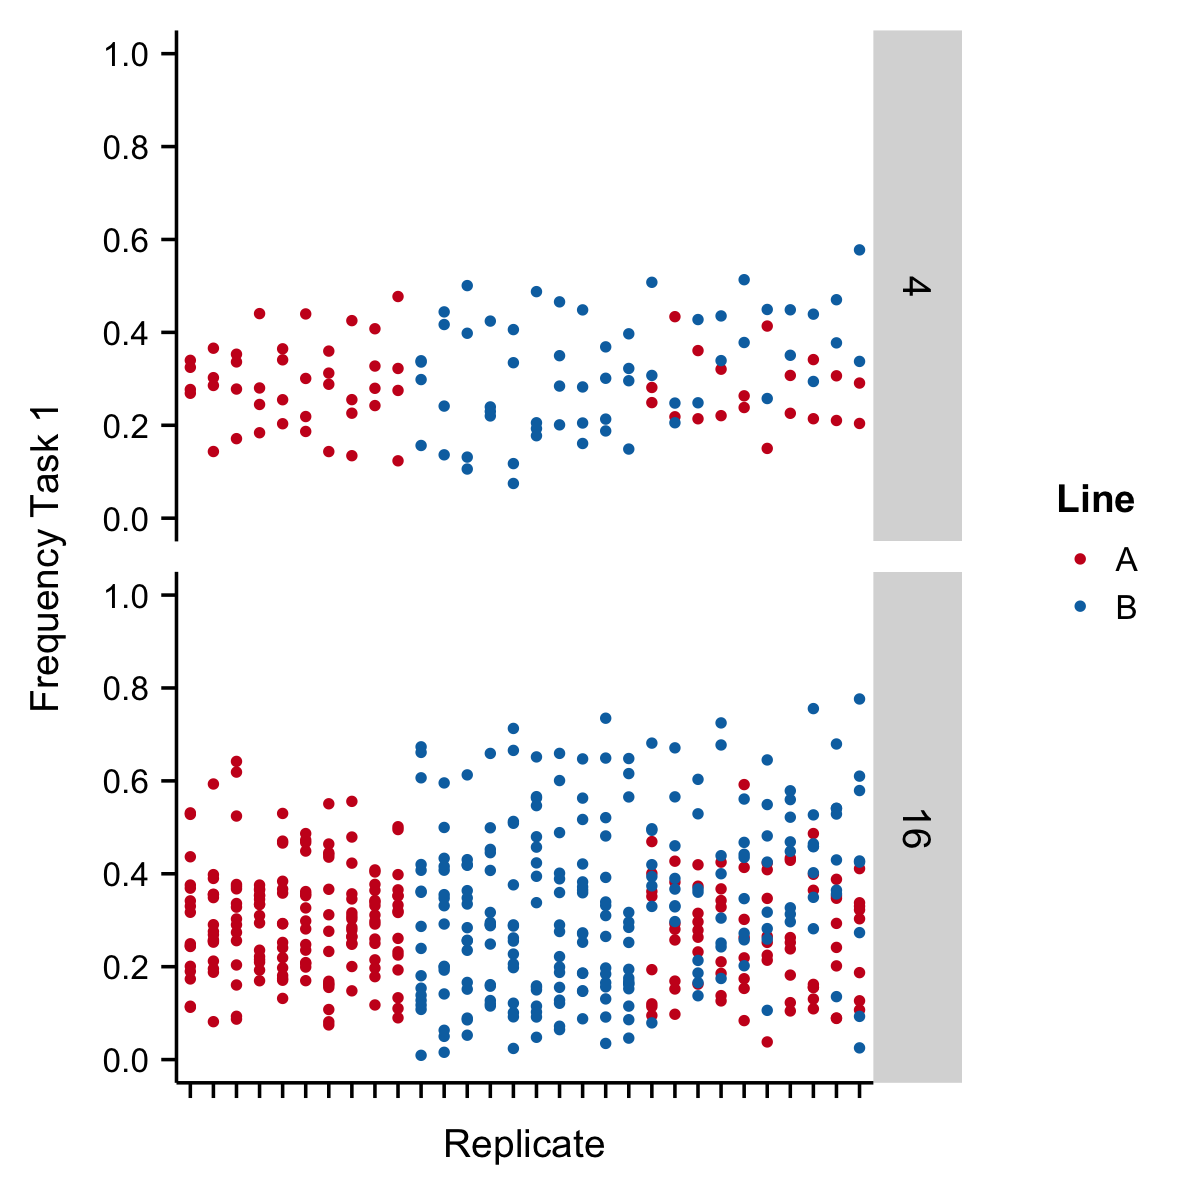
\includegraphics[width=.4\linewidth]{Diff_Etas_HighB.png}
	\caption{Varying threshold stochasticity ($\eta$) by line. The parameter values are identical to those in the base case, with the exception of line-specific threshold slope parameters, $\eta^A = 7, \eta^B = 14$.
	\vspace{-5pt}} 
%	\\\hspace{0pt}\\
%\textbf{Observation}: 	
	\label{fig:varyetaAB}
\end{figure}

\subsection{Varying threshold variance $\sigma$ by line}\vspace{-5pt}

\begin{figure}[H]
	\centering
	\includegraphics[width=.4\linewidth]{{AThreshM_10.00_10.00_AThreshSD_0.10_0.10_BThreshM_10.00_10.00_BThreshSD_0.30_0.30_deltas_0.60_0.60_threshSlope_7_7_Aalpha_2.00_2.00_Balpha_2.00_2.00_quitP_0.20_0.20}.png}
	\caption{Varying threshold variance ($\sigma$) by line. The parameter values are identical to those in the base case (Fig.~\ref{fig:base}) with the exception of line-specific threshold variances, $\sigma^A = 0.1, \sigma^B = 0.3$. 
%	\\\hspace{0pt}\\
%\textbf{Observation}: Varying the threshold variance \textit{does not} appear to alter the mean frequency of performing task 1.
%\\\hspace{0pt}\\
%If we do not observe a difference in the variance of task performance between the two types of ants (in all three experiments), then it is unlikely that this parameter governs the behavior of the single-line vs. mixed colonies. {\color{black}Whether we observe such a difference or not should be able to be answered empirically (the data already there, additional statistical tests needed).}
\vspace{-10pt}}
	\label{fig:varysigmaAB}
\end{figure}

Varying the threshold variance \textit{does not} appear to alter the mean frequency of performing task 1. {\color{black}Additionally, the data do not appear to show significant differences in the variance of RMSD between A-only and B-only colonies---although additional statistical tests might be needed to confirm this.}
In this case, it seems biologically implausible that variation in $\sigma$ governs the behavior of the single-line vs. mixed colonies.


\section{Additional results: varying parameters by task only}\label{sec:bytask}

\subsection{Parameters values tested}

\begin{table}[H] \small
  \begin{center}
    \begin{tabular}{|c|>{\centering}m{0.5in}|>{\centering}m{1.1in}|m{3.8in}|} 
      \hline
      \textbf{Parameter} & \textbf{Varied?} & \textbf{Model value(s)} & \textbf{Notes / Biological interpretation} \\ \hline
      $n$ & Fixed & $n = 4, 16$ & Based on colony sizes used in the mixing experiments \\ \hline
      $m$ & Fixed & $m = 2$ & For simplicity; no compelling reason to change from \cite{ulrich2018} \\ \hline
      $\delta$ & By task & $\delta_1 = 0.6, \delta_2 = 1.8 $ & Demand for task 2 increases more rapidly than that for task 1; $\delta$ could capture the difference between A larvae vs. B larvae? \\ \hline
      $\alpha$ & By task  & $\alpha_1 = 2,\alpha_2 = 6$ & Ants are more efficient at task 2 than at task 1 \\ \hline
      $\mu$ & By task  & $\mu_1 = 10,\mu_2 = 20 $ & The mean threshold for task 2 is higher than that for task 1\\ \hline
      $\sigma$ & By task & $\sigma_1 = 0.1, \sigma_2 = 0.3$ & Ants vary more in their internal thresholds for task 2 than for task 1 \\ \hline
      $\eta$ & Fixed & $\eta = 7$ & Stochasticity in behavior seems inherent to the ants, not tasks\\ \hline
      $\tau$ & Fixed & $\tau = 0.2$ & 
%      Ants have a shorter period for task 2 relative to task 1 (e.g., task 2 is more taxing so they need to take more breaks) 
      \\ \hline
    \end{tabular}
    \caption{Varying parameters by task.}
    \label{tab:table3}
  \end{center}
\end{table}

\subsection{Varying task performance efficiency $\alpha$ by task}

\begin{figure}[H]
	\centering
	\includegraphics[width=.4\linewidth]{{New_AThreshM_10.00_10.00_BThreshM_10.00_10.00_deltas_0.60_0.60_threshSlope_7_Aalpha_2.00_6.00_Balpha_2.00_6.00_quitP_0.20}.png}
	\caption{Varying task performance efficiency ($\alpha$) by task. The parameter values are identical to those in the base case (Fig.~\ref{fig:base}) with the exception of task-specific efficiencies, $\alpha_1 = 2, \alpha_2 = 6$. 
	% alpha_bug fixed
}
	\label{fig:varyalpha12}
\end{figure}

\subsection{Varying mean threshold $\mu$ by task}

\begin{figure}[H]
	\centering
	\includegraphics[width=.4\linewidth]{{AThreshM_10.00_20.00_BThreshM_10.00_20.00_deltas_0.60_0.60_threshSlope_7_Aalpha_2.00_2.00_Balpha_2.00_2.00_quitP_0.20}.png}
	\caption{Varying mean threshold ($\mu$) by task. The parameter values are identical to those in the base case (Fig.~\ref{fig:base}) with the exception of task-specific mean thresholds, $\mu_1 = 10, \mu_2 = 20$. 
%	\\\hspace{0pt}\\
%\textbf{Observation}: 
%No visible change compared to the base case. Our intuitive interpretation is that the stimulus for the task with the higher mean threshold (in this case task 2) decreases more slowly, which means that the ants have a smaller probability for performing that task (task 2) but over a longer period of time.
}
	\label{fig:varymu12}
\end{figure}

No visible change compared to the base case. Our intuitive interpretation is that the stimulus for the task with the higher mean threshold (in this case task 2) decreases more slowly, which means that the ants have a smaller probability for performing that task (task 2) but over a longer period of time.

\subsection{Varying threshold variance $\sigma$ by task}

\begin{figure}[H]
	\centering
	\includegraphics[width=.4\linewidth]{{AThreshM_10.00_10.00_AThreshSD_0.10_0.30_BThreshM_10.00_10.00_BThreshSD_0.10_0.30_deltas_0.60_0.60_threshSlope_7_7_Aalpha_2.00_2.00_Balpha_2.00_2.00_quitP_0.20_0.20}.png}
	\caption{Varying threshold variance ($\sigma$) by task. The parameter values are identical to those in the base case (Fig.~\ref{fig:base}) with the exception of task-specific threshold variances, $\sigma_1 = 0.1, \sigma_2 = 0.3$. 
%	\\\hspace{0pt}\\
%\textbf{Observation}: 
%Changing the threshold variance for one task (task 2 in this case) affects the performance frequency of the other task (task 1) as well, as expected. Variance in task 1 performance frequency is greater than in the base case.
}
	\label{fig:varysigma12}
\end{figure}

The variance in task 1 performance frequency is greater than in the base case.
As we expected, changing the threshold variance for one task (task 2 in this case) affects the performance frequency of the other task (task 1) as well. 

\subsection{Varying task demand rate $\delta$ by task}

\begin{figure}[H]
	\centering
	\includegraphics[width=.4\linewidth]{{AThreshM_10.00_10.00_BThreshM_10.00_10.00_deltas_0.60_1.80_threshSlope_7_Aalpha_2.00_2.00_Balpha_2.00_2.00_quitP_0.20}.png}
	\caption{Varying task demand rate ($\delta$) by task. The parameter values are identical to those in the base case (Fig.~\ref{fig:base}) with the exception of task-specific demand rates, $\delta_1 = 0.6, \delta_2 = 1.8$. \\\hspace{0pt}\\
%\textbf{Observation}: 
}
	\label{fig:varydelta12}
\end{figure}



%\begin{figure}[H]
%	\centering
%	\includegraphics[width=.4\linewidth]{{AThreshM_10.00_10.00_BThreshM_10.00_10.00_deltas_1.80_1.80_threshSlope_7_Aalpha_2.00_2.00_Balpha_2.00_2.00_quitP_0.20}.png}
%	\caption{Higher task demand rate ($\delta$) for both tasks compared to the base case, with $\delta_1 = \delta_2 = 1.8$. \\\hspace{0pt}\\
%%\textbf{Observation}: 
%}
%	\label{fig:varydeltaextra}
%\end{figure}
\end{appendices}


\end{document}
%%%%%%%%%%%%%%%%%%%%%%%%%%%

